\chapter{Adventuring and Downtime}
This chapter covers rules about adventuring and what goes on between adventures.

\section{Leveling Up}
When your GM decides you have enough experience and you have time to rest, you main gain a level. You get the following benefits:

\begin{itemize}
	\item Your max health increases by 10\% of your Endurance.
	\item You may distribute 10 points among your major skills, but no more than 5 into any single one.
	\item You may distribute 10 points among your minor skills, but no more than 3 into any single one.
	\item Once your skill points are distributed, select three primary attributes to increase. This is where the governing attributes of skills come in: if you have not raised any skills governed by an attribute, a selected attribute will increase by only one point. If you have put 1-4 points into skills governed by that attribute, it increases by 2 points. If you have put 5-7 points in skills governed by that attribute, it increases by 3 points. If you have put 8-9 points in skills governed by that attribute, it increases by 4 points. Finally, if you have put 10 or more points into skills governed by an attribute, it increases by 5 points.
\end{itemize}

\begin{tcolorbox}
\textbf{Example}: Ingvar Iron-Fist the Nord Barbarian increases his level from 1 to 2. His Endurance is 55, so his max health increases by 5 points. He puts 4 skill points into Blunt, 2 into Athletics and 4 into Light Armor for his major skills. For his minors, he puts 3 into Acrobatics, 3 into Sneak, 3 into Marksman and 1 into Speechcraft. He selects the attributes Strength, Speed and Endurance to increase. He has put 4 points into Strength skills, so his Strength goes up by 2 points. He has put 10 points into Speed skills, so his Speed goes up by 5. He has put no points into Endurance skills, so his Endurance goes up by 1.
\end{tcolorbox}

\section{Encumbrance}
You are able to carry a weight equal to $5*\text{Strength}$ in pounds. If you exceed this weight, you are encumbered and cannot move. Mounts do not have this limitation, but don't get crazy. There are also spells which can alter encumbrance limits.

\section{Travel}
Characters can travel 24 miles per day, assuming they are traveling for a full 8 hours. Each additional hour of travel after that risks exhaustion. Make a percentile roll at the end of each additional hour. You must roll less than or equal to $50-5*\text{extra hours}$ or increase your exhaustion level.\\

Mounts are able to move double speed for one hour, but they must rest an hour before they can do so again. Vehicles are limited by specific speeds, but they may be able to travel for over 8 hours a day without penalty.\\

Difficult terrain halves travel speed while it is traversed.

\begin{figure}[H]
	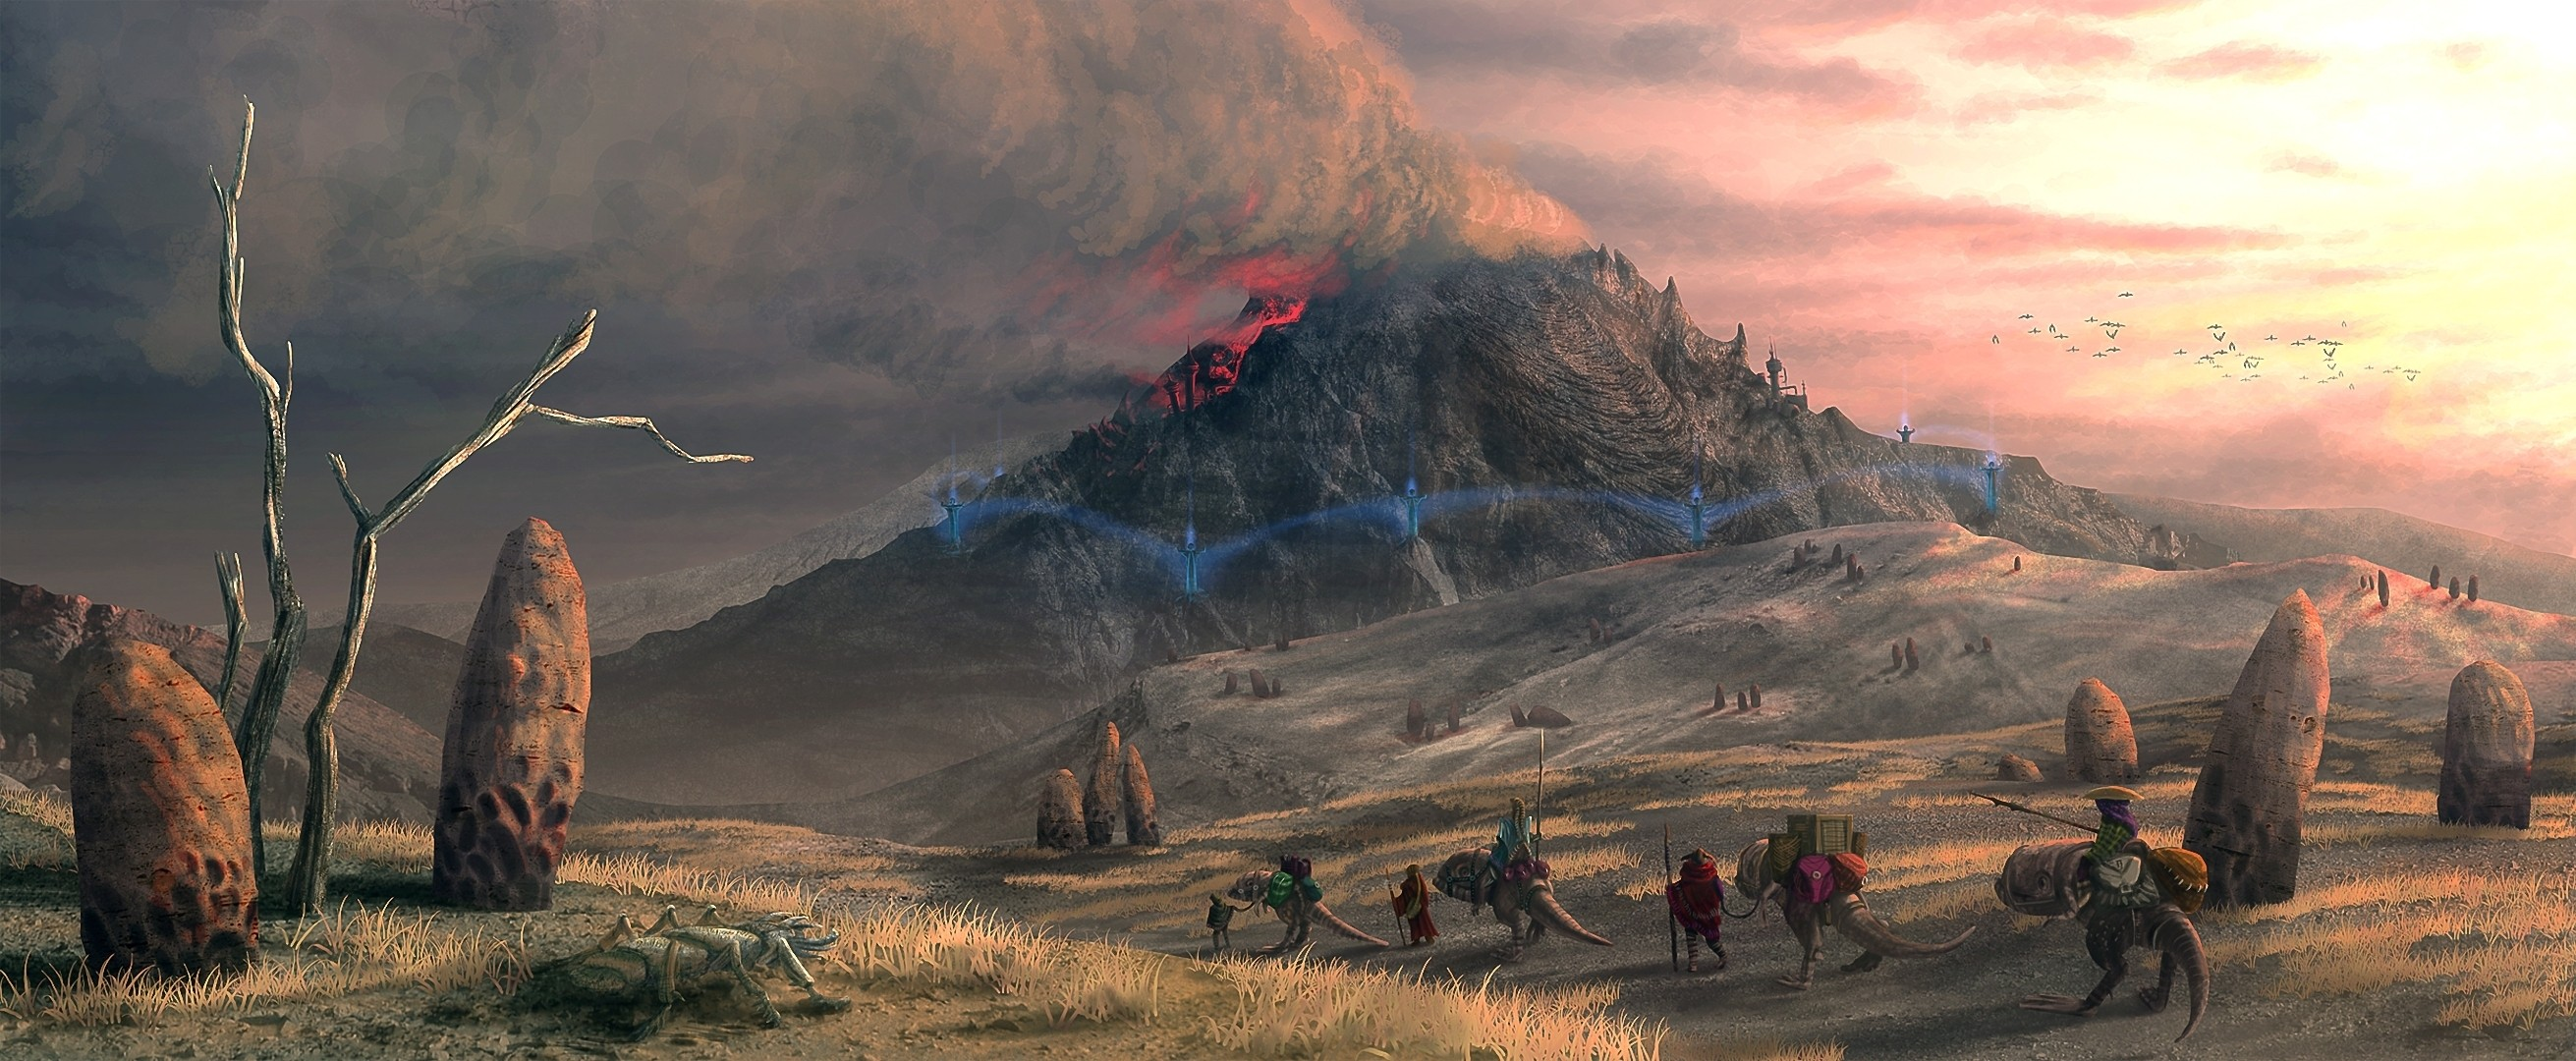
\includegraphics[width=\textwidth]{Morrowind.png}
\end{figure}

\section{Resting}
A short rest is defined by a period of at least an hour during which time you do nothing more strenuous than eat, drink, tend to wounds or other physically restful tasks. Your health, magicka and stamina are fully recovered after short rest, though you may not decrease your level of exhaustion. If you have enough experience, you may gain a level during this time.\\

A long rest is a period spanning at least 8 hours of sleep and light activity including no more than 2 hours of standing watch. You gain all the benefits of a short rest and may decrease your exhaustion by one level. You must complete a long rest once per day with access to sufficient food and drink or else your exhaustion will increase a level.

\section{Survival}
Survival in the Elder Scrolls Tabletop relies on a combination of roleplaying and skill checks. There are no "Surivival" skills like there are in other RPGs; rather, the effects of what you do will be decided by which actions you take and what skills you character possesses. Alchemy, for example, may be useful to determine whether plants are safe for eating. Sneak may be useful to hunt for food. Acrobatics could be useful to get to a vantage point and find running water. Improvise, and wilderness survival will still be a fun challenge.

\subsection{Food}
A grown humanoid needs a pound of food a day to survive. Eating half a pound of food in a day will count as a half-day without food. You can go without food for a number of days equal to $3+0.05Endurance$. After this point, each full day you go without food will increase your exhaustion by one level. A normal day of eating resets the count.

\subsection{Water}
A character needs a gallon of water a day, or two if the weather is hot and dry. Characters who only drink half that in a day must roll less than or equal to $75-0.05Endurance$ or suffer a level of exhaustion. Characters who get even less gain an exhaustion level automatically. If the character already has at least one exhaustion level, they gain two exhaustion levels due to lack of water.

\section{Vision}
Most tasks require vision to some extent. \textit{Lightly obscured} areas provide a bonus die to Sneak checks. \textit{Heavily obscured areas} obstruct vision entirely imposing blindness on everyone in them. Certain weather conditions may obscure vision. Bright light does not obscure, dim light obscures lightly, and darkness obscured heavily. Vision-altering effects may change how light levels affect your character.

\section{Lockpicking}
Picking locks depends on your Security skill. As long as you have a lockpick, you can attempt to pick a lock. You can automatically pick locks at your skill level as defined in the mastery perk chart. You may attempt to pick higher level locks, but you must roll to succeed. If the lock is one level higher than your automatic success level, you need a normal success. If the lock is two levels higher, you need a hard success. If the lock is three levels higher, you need an extreme success. If the lock is four levels higher, it is impossible.

\section{Traps}
You're likely to encounter traps whenever you venture into a dungeon. Detecting traps works using two skills: Sneak and Security. Having a high Sneak skill allows you to set well-hidden traps since you know a lot about hiding things from sight. Security is used to detect the presence of traps and successfully disarm them. Thus, attempting to set traps for other characters will rely on your Sneak and attempting to detect traps before you run into them will depend on your Security.

\section{Different Types of Movement}

\subsection{Climbing and Swimming}
While climbing or swimming, each foot moved costs an extra foot of your movement (or an extra 2 feet in difficult terrain). If conditions are especially hostile, you may be required to make an Athletics or Acrobatics check.

\subsection{Jumping}
If you have at least 10 feet to get a running start, you can long jump a distance in feet equal to one-fifth of your Acrobatics or Strength, whichever is higher. Standing long jumps can only cover half that distance. Each foot you clear costs a foot of movement. You may be required to make an Acrobatics check to jump farther than you normally can.

If you have at least 10 feet to get a running start, you can high jump a height in feet equal to 3+5\% of your Acrobatics or Strength, whichever is higher. Standing high jumps can only jump half as high. You may be required to make an Acrobatics check to jump higher than you normally can. You can extend you arms to reach higher while jumping.

\subsection{Falling}
Gravity exists in the world of Elder Scrolls, and you will get hurt if you fall down. Experienced acrobats are able to handle falls better than the average person, however. For every 10 feet you fall, you suffer 4d20 health damage, ignoring armor. For every 25 points in your Acrobatics skill, this distance increases by 5 feet.

\section{Social Interaction}
Your Personality attribute along with various factors will set an NPC's initial disposition toward you. Rather than rolling Speechcraft to determine whether an NPC is convinced of specific things, Speechcraft checks allow you to increase your disposition with an NPC by varying amounts depending on your level of success. The resulting disposition level may be high enough that the NPC is willing to give you something you ask for, depending on what it is.\\

The limits on Speechcraft checks depend on your roleplaying: you may not attempt a roll for the same oratory tactic twice in the same conversation. You also cannot make more than three Speechcraft checks to improve disposition in a single conversation, meaning you must take time to build up a positive rapport with an NPC unless you are very skilled or lucky. Speechcraft mastery perks improve your ability to do this.\\

NPC disposition may be affected by circumstance. If you cannot improve disposition well enough in a single conversation, you might try doing something that the NPC will like. Gifts of money or valuable items will help as well, but be sure to give a gift appropriate to the NPC's wealth and station, or else they may find it insulting!

\section{Downtime}

\subsection{Lifestyle Expenses}
Between adventures, you need to pay the expenses demanded by your lifestyle. It is up to you what sort of lifestyle you wish to live, so long as you can afford it. This has no mechanical effect, but it may change how NPCs are disposed to react to you. The local nobility might give you more attention if you are known to live a wealthy lifestyle. Lifestyle costs:

\begin{center}
{
\rowcolors{2}{gray!25}{white}
\begin{tabular}{ll}
	\textbf{Wretched} (Inhumane) & 0 Septims/day\\
	\textbf{Squalid} (Basic shelter) & 10 Septims/day\\
	\textbf{Poor} (Sufficient but unpredictable) & 25 Septims/day\\
	\textbf{Modest} (Stable home) & 100 Septims/day\\
	\textbf{Comfortable} (Middle-class) & 200 Septims/day\\
	\textbf{Wealthy} (Good businessman) & 500 Septims/day\\
	\textbf{Aristocratic} (Old money) & At least 1000 Septims/day\\
\end{tabular}
}
\end{center}

\subsection{Work}
If you are working a profession, it is assumed you earn and spend money on lifestyle expenses to support a modest living. If you are affiliated with an organization that can provide gainful employment (e.g. Fighters Guild, Mages Guild, Thieves Guild or another such thing), you can support a comfortable lifestyle. If you have a high skill in Mercantile, you can support a wealthy lifestyle.

\section{Research}
In the Elder Scrolls tabletop, there are no knowledge skills to determine whether your character knows something already. Instead, the GM will give you any information your character should reasonably know based on backstory information, and new information will be learned from NPCs and interacting with the world. Sometimes, you may be called upon to do in-depth research taking several days. If your character is capable of performing this research and has the time, you may do so. Otherwise, it is best to enlist the services of a scholar and then wait.

\begin{figure}[h]
	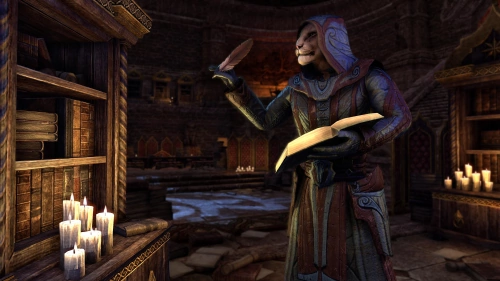
\includegraphics[width=\textwidth]{scholar.png}
\end{figure}

\section{Disease}
During your adventure, you may be unfortunate enough to contract a disease. Diseases inflict various penalties to your stats and may render you unable to work during downtime. There are three methods of recover: potions, altars and rest. Ingesting a disease cure potion or praying at an altar of the Divines will immediately cure most diseases, leading many afflicted to seek out alchemists and priests. Those who cannot access either may roll percentile against $25+0.05*\text{Endurance}$ every three days of rest to end the disease.

\section{Conditions}
Conditions alter your abilities in certain ways. They can arise as a result of combat techniques, spells or natural laws.

\subsection{Blinded}
A blinded creature cannot see and automatically fails and sight-based check. Attack rolls against a blinded creature have a bonus die, and attack rolls made by the creature have a penalty die.

\subsection{Calmed}
A calmed creature has no strong emotions and will not attack anyone or move. Calmed creatures are still aware, and being attacked will end their calm state.

\subsection{Charmed}
A charmed creature will not take action against the charmer. The charmer has a bonus die on Speechcraft checks with the creature for the duration.

\subsection{Deafened}
A deafened creature cannot hear and automatically fails any hearing-based check. Everyone is deafened to the movements of a Muffled creature.

\subsection{Exhausted}
Exhaustion comes in multiple levels. Each level includes all the penalties of the levels prior to it. Finishing a long rest makes your exhaustion level go down by 1, assuming you have access to sufficient food and drink.\\

Levels of exhaustion:

\begin{enumerate}
	\item Penalty die on all skill rolls.
	\item Movement halved.
	\item Penalty die on all attack and reaction rolls.
	\item Max health halved.
	\item Movement is 0.
	\item Death.
\end{enumerate}

\subsection{Frenzied}
A frenzied creature is blinded by consuming rage and cannot think clearly or distinguish friend from foe. It will attack the nearest creature it can, indiscriminately.

\subsection{Frightened}
A frightened creature has a penalty die on all attack and skill rolls made while its source of fear is within sight and cannot willingly move closer to the source of its fear.

\subsection{Grappled}
A grappled creature has no movement.

\subsection{Incapacitated}
An incapacitated creature cannot move, use actions or reactions.

\subsection{Invisible}
The creature is impossible to see without magic or special tactics. While invisible, a creature is considered heavily obscured and has a bonus die on attack rolls while attack rolls made against it have a penalty die.

\subsection{Paralyzed}
A paralyzed creature is incapacitated and cannot move or speak. Attacks against a paralyzed creature get a bonus die, and any attacks made within 5 feet are automatically critical hits.

\subsection{Poisoned}
A poisoned creature takes a penalty die to attack and skill rolls.

\subsection{Prone}
The creature can only move by crawling, unless it stands up. It takes a penalty die to attacks it makes, and attacks made against it get a bonus die if the attacker is within 5 feet. Otherwise, attacks made against it get a penalty die.

\subsection{Recoiled (AKA Staggered)}
The creature is momentarily set off balance and must use its next action to recover. A recoiled creature will gain increased resistance to recoil briefly after regaining balance.

\subsection{Unconscious}
As with Paralyzed, but the creature also drops what it is holding, falls prone, and recovers stamina at a rate of 60/round. If the unconsciousness is induced by stamina loss, the creature regains consciousness when its stamina is non-negative.
